To support the GPGPU-Sim functional model, a number of the simulator's overloaded
CUDA Runtime API calls were updated. Several functions that originally assumed
the application and simulator were within the same address space now support them being
decoupled. Initialization functions, such as \texttt{\textunderscore \textunderscore
cudaRegisterFatBinary}, now take paths to the original application to obtain the PTX
assembly of CUDA kernels.


   \begin{figure}[!htb]
      \centering
      \setlength{\abovecaptionskip}{6pt plus 1pt minus 1pt}
      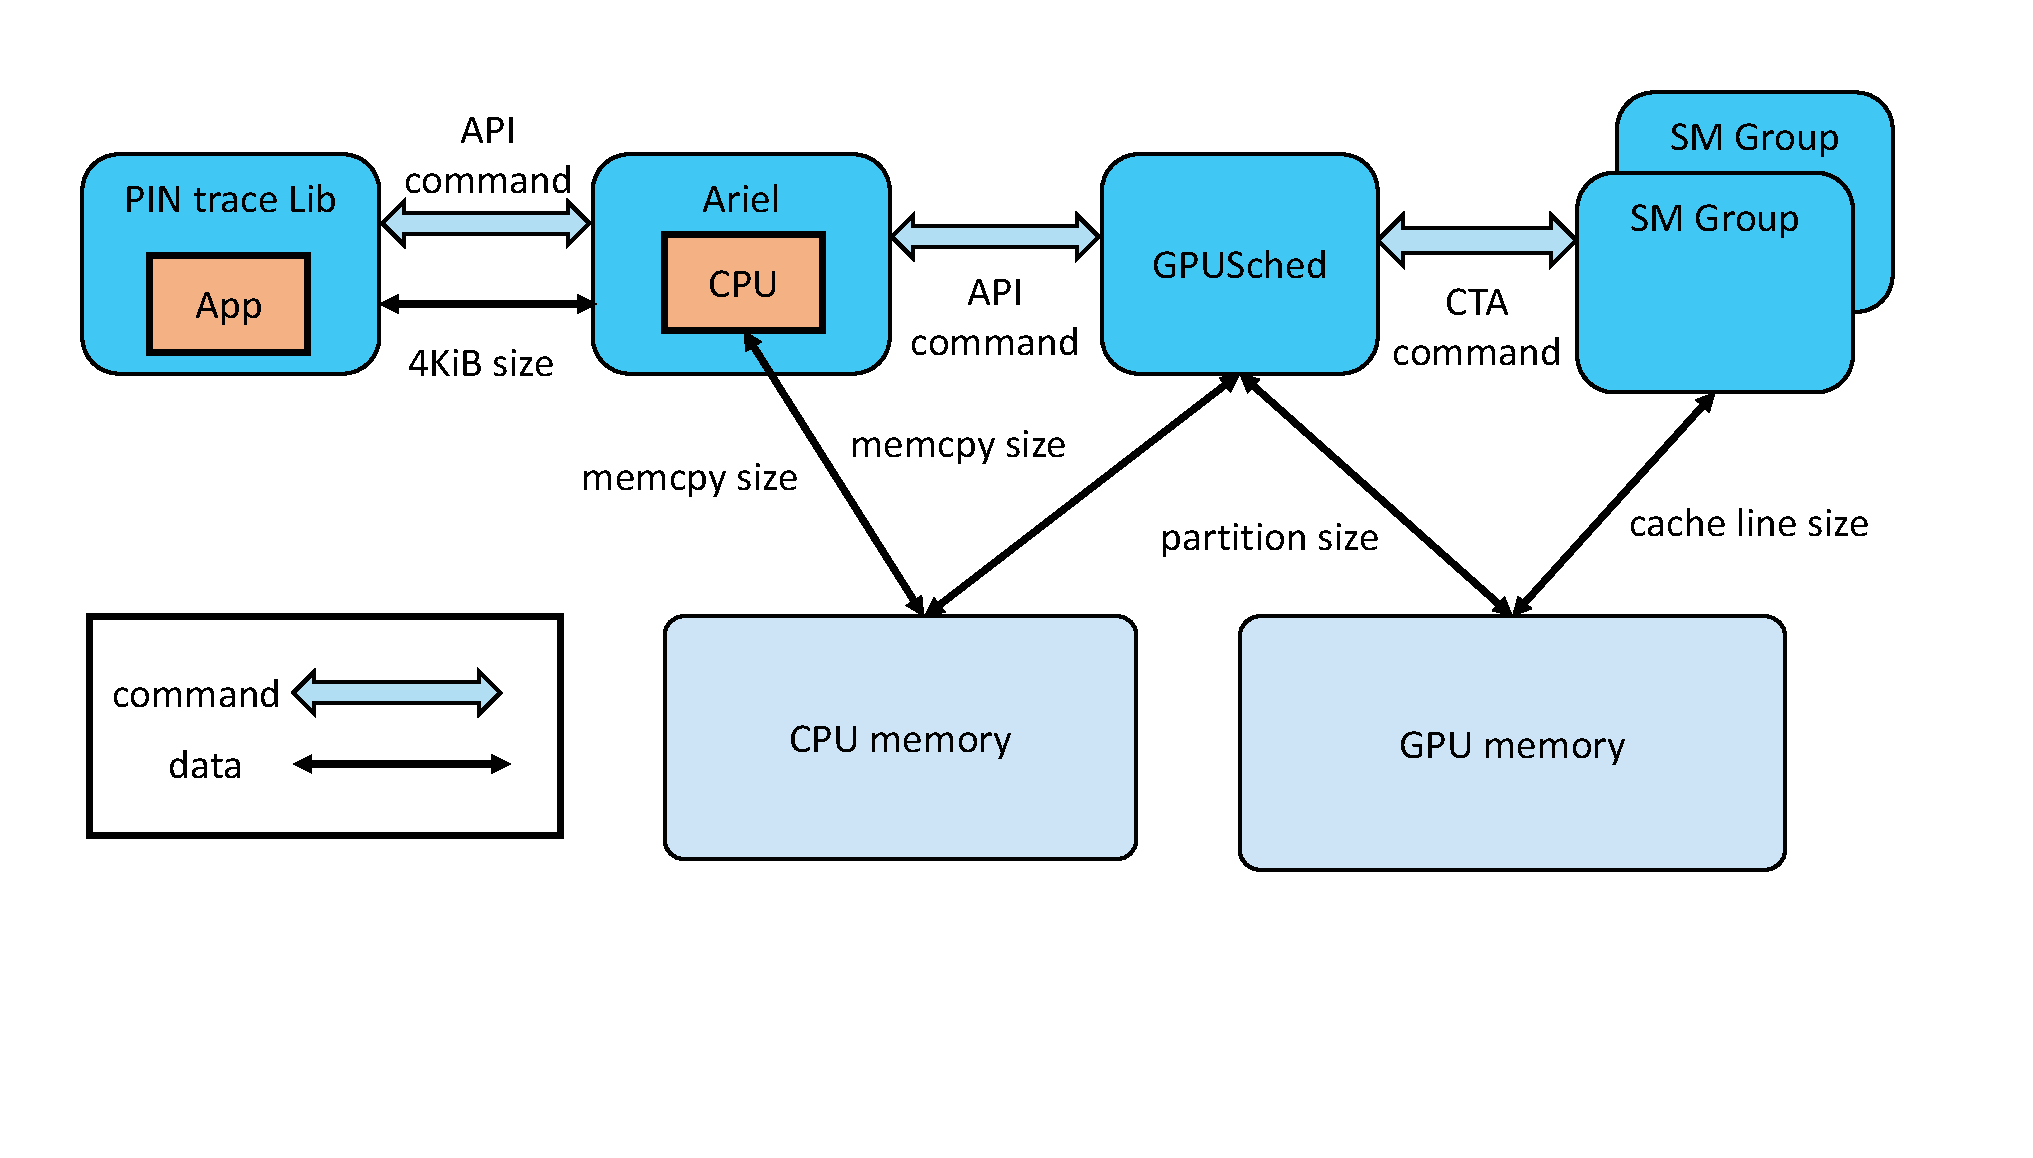
\includegraphics[width=.90\textwidth,keepaspectratio]{figures/transfer_flow.eps}
      \captionsetup{width=.75\textwidth}
      \caption{Data transfer flow for functional simulation}
      \label{fig:gpu_transfer_model}
   \end{figure}

Supporting the functional model of GPGPU-Sim also requires transferring values
from the CPU application to the GPU memory system. This is solved by leveraging
the link between CPU/GPU and memory hierarchy from SST, as shown in
\ref{fig:gpu_transfer_model}. Before actually storing values to memory, appropriate 
CPU memory and GPU memory spaces need to be allocated. As a matter of fact, both CPU memory 
and GPU memory are physically pre-allocated, and their sizes are set in the configuration file. 
Therefore, the rest of "allocation" just needs to avoid collision. A simple way to do this is
keeping a pointer to the current boundry of heap but at the cost of unable to free memory chunks. 
CPU memory allocation is done by Ariel in the CPU simulation -- an option argument is set inside 
configuration file to intercept memory allocation, but other load/store instructions are ignored 
to reduce simulation time. \texttt{malloc} is sent from application to Ariel and the MMU of Ariel takes 
over to settle page allocation; while GPU memory allocation is completed by the 
GPU Scheduler. Unlike the Ariel, there's no MMU inside the GPU so the only thing \texttt{cudaMalloc} 
needs to do is to move the pointer.

Data are transferred from the application to Ariel through
inter-process communication tunnels when \texttt{cudaMemcpy} is called. 
Ariel then communicates with the GPU scheduler through
the CPU memory. The GPU scheduler then writes the data to the GPU memory. When an SM
requests a piece of data, the SM accesses the GPU memory for it.
The tunnels utilize 4KiB size as the granularity, while the CPU and the GPU Scheduler
employ larger size non-cacheable requests to access to the CPU memory. When it comes to
GPU memory, some particular attention needs to be paid. The GPU Scheduler communicates with 
the GPU memory in partition size because only one partition can be accessed at a single time. 
The SM transfers data to/from the GPU memory in cache line size because store/load 
instructions manipulate data in cache line granularity (more details in next paragraph). 

To model GPU performance, the memory system of the public GPGPU-Sim is
completely removed. Instead, all accesses to GPU memory are sent though SST
links to the MemHierarchy interface. As Figure \ref{fig:gpu_mem_model} shows, a
multi-level cache hierarchy is simulated with the shared L2 sliced between
different memory partitions, each with its own memory controller. Several
backend timing models have been configured and tested, including SimpleMem,
SimpleDRAM, TimingDRAM, and CramSim \cite{healy2017}; CramSim will be used to
model the HBM stacks in the more detailed performance models. We have created an
initial model for the GPU system similar to that found in an Nvidia Volta. The
configuration for the GPU, CramSim and Network components is shown in Listing
\ref{lst:sst_config}.


\lstdefinelanguage{mooCows}
{
  basicstyle={\small\ttfamily},
  columns=flexible,
  tag=[s]{[]},
  tagstyle=\color{dkgreen}\bfseries,
  usekeywordsintag=true
}[html]

\lstset{frame=tb,
  language=mooCows,
  aboveskip=3mm,
  belowskip=3mm,
  showstringspaces=false,
  columns=flexible,
  basicstyle={\small\ttfamily},
  numbers=none,
  numberstyle=\tiny\color{gray},
  breaklines=true,
  breakatwhitespace=true,
  tabsize=3
}

\lstinputlisting[caption=Sample SST-GPGPU Configuration, label=lst:sst_config]{figures/config}

